%CS-113 S18 HW-3
%Released: 2-March-2018
%Deadline: 16-March-2018 7.00 pm
%Authors: Abdullah Zafar, Waqar Saleem.


\documentclass[addpoints]{exam}

% Header and footer.
\pagestyle{headandfoot}
\runningheadrule
\runningfootrule
\runningheader{CS 113 Discrete Mathematics}{Homework IV}{Spring 2018}
\runningfooter{}{Page \thepage\ of \numpages}{}
\firstpageheader{}{}{}

\boxedpoints
\printanswers
\usepackage[table]{xcolor}
\usepackage{amsfonts,graphicx,amsmath,hyperref,amssymb}
\hypersetup{
    colorlinks=true,
    linkcolor=blue,
    urlcolor=cyan,
}

\title{Habib University\\CS-113 Discrete Mathematics\\Spring 2018\\HW 4}
\author{$<your ID>$}  % replace with your ID, e.g. oy02945
\date{Due: 19h, 16th March, 2018}


\begin{document}
\maketitle

\begin{questions}



\question
\begin{parts}
  \part Prove that $1 = -1 \rightarrow 2 = 1$
  
  \begin{solution}
    % Write your solution here
  \end{solution}
  
  \part Let $a,b \in \mathbb{N}$. What's wrong with the following proof:
  \begin{align*}
  a &= b\\
  a^2 &= ab\\
  a^2 - b^2 &= ab - b^2\\
  (a-b)(a+b) &= (a-b)b\\
  a+b &= b\\
  a &= 0
  \end{align*}
  \begin{solution}
    % Write your solution here
  \end{solution}

  \part What's wrong with the following proof that shows $2^n = 1, n = \{0,1,2,...\}$, using strong induction on $n$:
  
  \textbf{Base step:} When $n=0, 2^0=1$, so the result holds.
  
  \textbf{Inductive step:} Suppose the result holds for $0\leq n \leq k$. We will show that it holds for $n=k+1$, i.e. that $2^{k+1}=1$.
  
  \begin{align*}
      2^{k+1} &= \frac{2^{2k}}{2^{k-1}}\\
      &= \frac{2^k.2^k}{2^{k-1}}\\
      &= \frac{1.1}{1}\\
      &= 1
  \end{align*}

  \begin{solution}
    % Write your solution here
  \end{solution}
\end{parts}

\question Buckminster Fuller once said: ``None of the world’s problems will have a solution until the world’s individuals become thoroughly self-educated."

The world is full of problems, but which ones should you focus on? According to \href{http://8000hours.org}{80000.org}, the most urgent problems are ``not only \textbf{big}, they're also \textbf{neglected} and \textbf{solvable} - the fewer people working on a problem, the easier it is to make a big contribution. An issue can be big but comparatively well-known and crowded, like climate change, or it can be small but neglected, like land use zoning reform, and therefore also worth considering."

We present a list of the biggest, most solvable and most neglected global issues that would benefit the most from your contribution. You are encouraged to read more about how these problems measure up at \href{https://80000hours.org/articles/cause-selection/}{8000hours.org}.
\begin{center}
\begin{tabular}{ c c c}
Biosecurity & Climate change & Promoting effective altruism\\\\
Institutional decision-making & Risk from AI & Nuclear Security\\\\
Developing world health & Land use reform & Factory farming
\end{tabular}
\end{center}

You are given a set of 9 global challenges - to which you may add one more of your choice - and three order relations on them: \textbf{NB}: ``not bigger than", \textbf{NS}: ``not more solvable than" and \textbf{NN}:``not more neglected than". Using all 10 challenges and your intuition, give unique answers for each of the following. (Well-formatted, syntactically sound answers are encouraged) 

\begin{parts}
\part A poset of width 5
\part A decomposition of size 4
\part A lattice
\part A totally-ordered set
\part A well-ordered set
\end{parts}

(You may refer to the \textbf{Appendix} for a list of definitions)


  \begin{solution}
    % Write your solution here
  \end{solution}
  
\question 
A poset $(R, \preccurlyeq)$ is \textbf{well-founded} if there is no infinite decreasing sequence of elements in the poset, i.e. elements $x_1, x_2, \cdots, x_n$ such that $\cdots \prec x_n \prec \cdots  \prec x_2 \prec x_1$. A poset $(R, \preccurlyeq)$ is \textbf{dense} if for all $x \in S$ and $y \in S$ with $x \prec y$, there is an element $z \in R$ such that $x \prec z \prec y$.

Show that the set of strings of lowercase English letters with lexicographic order is neither well-founded nor dense.


  \begin{solution}
    % Write your solution here
  \end{solution}

\question
     Let $S$ and $T$ be two partial orders on a set $A$. Define a new relation $R$ on $A$ by $(x,y)\in R$ iff both $(x,y) \in S$ and $(x,y) \in T$. Prove that $R$ is a partial order on $A$.

    
      \begin{solution}
    % Write your solution here
  \end{solution}

\question Your overly-attached girlfriend / boyfriend has concocted a cruel game to keep you around forever. The game involves piles of excuses - each pile twice as high as the last - of all the times you didn't hang out with them. Stacked in increasing order, the piles look truly endless! 

\begin{figure}[ht]
  \centering
  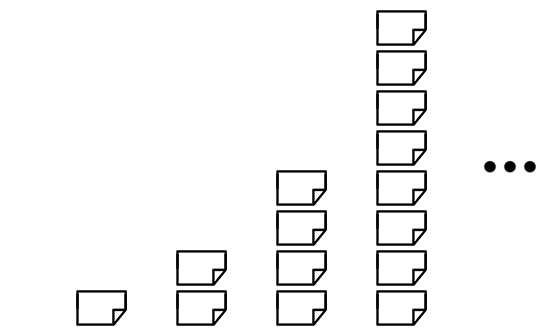
\includegraphics{excuses.png}
  \caption{That escalated quickly.}
  \label{fig:Piles of excuses}
\end{figure}

The game of \textbf{Gazillion Excuses} is a turn based 2-player game such that at each turn, a player removes a non-zero number of excuses from one of the piles. The player who removes the last excuse wins. Your partner thinks that a sufficiently large number of piles (think gazillion) would keep you playing forever. Little do they suspect that a Discrete Mathematician like yourself has formidable proof skills! Given that you are allowed to go first, \textbf{formally prove} that you will always win the game of Gazillion Excuses. 



\end{questions}

\end{document}